%==============================================================================
% Sjabloon onderzoeksvoorstel bachelorproef
%==============================================================================
% Gebaseerd op LaTeX-sjabloon ‘Stylish Article’ (zie voorstel.cls)
% Auteur: Jens Buysse, Bert Van Vreckem
%
% Compileren in TeXstudio:
%
% - Zorg dat Biber de bibliografie compileert (en niet Biblatex)
%   Options > Configure > Build > Default Bibliography Tool: "txs:///biber"
% - F5 om te compileren en het resultaat te bekijken.
% - Als de bibliografie niet zichtbaar is, probeer dan F5 - F8 - F5
%   Met F8 compileer je de bibliografie apart.
%
% Als je JabRef gebruikt voor het bijhouden van de bibliografie, zorg dan
% dat je in ``biblatex''-modus opslaat: File > Switch to BibLaTeX mode.

\documentclass{voorstel}

\usepackage{lipsum}
\usepackage{graphicx}
\graphicspath{ {./images/} }

%------------------------------------------------------------------------------
% Metadata over het voorstel
%------------------------------------------------------------------------------

%---------- Titel & auteur ----------------------------------------------------

% TODO: geef werktitel van je eigen voorstel op
\PaperTitle{De invloed van quantum computing op de industrie}
\PaperType{Onderzoeksvoorstel Bachelorproef 2019-2020} % Type document

% TODO: vul je eigen naam in als auteur, geef ook je emailadres mee!
\Authors{Jochen Dewachter\textsuperscript{1}} % Authors
\CoPromotor{xyz\textsuperscript{2}}
\affiliation{\textbf{Contact:}
  \textsuperscript{1} \href{mailto:jochen.dewachter@student.hogent.be}{jochen.dewachter@student.hogent.be};
  \textsuperscript{2} \href{mailto:xyz@xyz.com}{xyz@xyz.com};
}

%---------- Abstract ----------------------------------------------------------

\Abstract{
  Dat de wereld steeds slimmer wordt kan men niet meer ontkennen, denk maar aan Artificial Intelligence en Machine Learning bijvoorbeeld.
  Desondanks deze ingewikkelde technologiën zijn er nog steeds problemen waar de klassieke computer geen weet mee is.
  Ondertussen zijn er ook hiervoor oplossingen gevonden: Quantum computers.
  Ook al zit quantum computing nog in zijn babyjaren, zijn grote bedrijven hier meer en meer mee bezig.
  In dit onderzoek wordt er gekeken naar de invloed hiervan. Er wordt zowel naar de positieve impact op de industrie gekeken als naar de negatieve kanten.
  Dit wordt gedaan aan de hand van enkele van de belangrijkste problemen die men momenteel niet efficiënt kan oplossen op een klassieke computer of zelf op een supercomputer.
  Er wordt wordt een vergelijking gedaan tussen:
  \begin{itemize}
    \item De tijdscomplexiteit.
    \item De ruimtecomplexiteit.
    \item De invloed van extra parameters op tijdscomplexiteit.
  \end{itemize}
  Deze vergelijking is steeds tussen hetzelfde algoritme in een klassieke computer en een quantumcomputer.
  Naast de karakteristieken van quantumcomputer wordt er ook nog onderzocht of de belangrijkste bedrijfprocessen van tegenwoordig weldegelijk efficiënter uitgevoerd kunnen worden.
  Dit onderzoek zal de positieve invloed van quantum computing op de industrie weergeven, maar ook de negatieve effecten zodanig dat men in de toekomst hierop kan anticiperen.
}

%---------- Onderzoeksdomein en sleutelwoorden --------------------------------
% TODO: Sleutelwoorden:
%
% Het eerste sleutelwoord beschrijft het onderzoeksdomein. Je kan kiezen uit
% deze lijst:
%
% - Mobiele applicatieontwikkeling
% - Webapplicatieontwikkeling
% - Applicatieontwikkeling (andere)
% - Systeembeheer
% - Netwerkbeheer
% - Mainframe
% - E-business
% - Databanken en big data
% - Machineleertechnieken en kunstmatige intelligentie
% - Andere (specifieer)
%
% De andere sleutelwoorden zijn vrij te kiezen

\Keywords{Quantum Computing. Quantum -- industrie} % Keywords
\newcommand{\keywordname}{Sleutelwoorden} % Defines the keywords heading name

%---------- Titel, inhoud -----------------------------------------------------

\begin{document}

\flushbottom % Makes all text pages the same height

\maketitle % Print the title and abstract box

\tableofcontents % Print the contents section

\thispagestyle{empty} % Removes page numbering from the first page

%------------------------------------------------------------------------------
% Hoofdtekst
%------------------------------------------------------------------------------

% De hoofdtekst van het voorstel zit in een apart bestand, zodat het makkelijk
% kan opgenomen worden in de bijlagen van de bachelorproef zelf.
%---------- Inleiding ---------------------------------------------------------

\section{Introductie} % The \section*{} command stops section numbering
\label{sec:introductie}

In dit onderzoek wordt de impact onderzocht van quantumcomputers op de industrie.
Op dit moment bestaan er 3 soorten computers: de klassieke computer, supercomputers en de quantumcomputer.
De klassieke computer kent iedereen en een supercomputer is hier eigenlijk een veel betere variant van: deze hebben meer rekenkracht, maar de principes blijven hetzelfde.
Nu zijn er nog steeds problemen die we niet efficient kunnen oplossen met onze computers.
Voorbeelden hiervan zijn: simulaties van molecules en quantumfysische begrippen, RSA (hèt encryptiealgoritme dat in transacties gebruikt wordt), zoeken in databanken(deze databanken hebben miljoenen entries), enz.
Het probleem zit niet bij de kracht van de tegenwoordige computers, maar in de tijd die een klassieke computer nodig heeft om een proces uit te voeren.
Dit komt omdat een klassieke computer alles 1 voor 1 moeten overlopen en verwerken en hierbij kunnen quantumcomputers van pas komen.

%---------- Stand van zaken ---------------------------------------------------

\section{State-of-the-art}
\label{sec:state-of-the-art}

Een klassieke computer werkt met bits: een 0 of een 1. In een computer wordt een bit gemaakt door een transistor.
Dit is eigenlijk gewoon een kleine schakelaar waar elektriciteit door gaat.
De transistor kan dan open staan en het signaal door laten (een één) of toe zijn en het signaal tegen houden (een nul).
Door middel van verschillende transistoren aan elkaar te koppelen onstaat een chip en kunnen er complexe bewerkingen uitgevoerd worden.
De transistor is dus de belangrijkste bouwsteen van de hedendaagse computer. Hoe beter de computer moet zijn, hoe beter de chip ofwel hoe meer transistoren.
Ieder jaar worden onze chips beter, maar niet groter. Het is zelfs zo dat volgens de Wet van \textcite{Moore1965} iedere 2 jaar het aantal transistoren verdubbeld wordt op een chip.
Nu kan dit enkel zo zijn doordat onze transistoren kleiner worden door de steeds verbeterende technologie en dit is inderdaad zo, de transistor is van enkele centimeters groot gekrompen naar enkele nanomters groot.
Maar dit kan niet blijven doorgaan. Zo is er berekend geweest dat de Wet van \textcite{Moore1965} nog tot rond 2036 zou gelden\autocite{Powell2008}.  Momenteel is een transistor zodanig klein dat als men nog veel kleiner zou gaan, een elektron (een negatief geladen deeltje waardoor electriciteit kan werken) door de transistor door kan gaan.
Het laatstgenoemde effect wordt ook wel het Tunneleffect genoemd. Normaal gezien kan een electron niet door de potentiaalbarricade van een transistor, maar door het golfgedrag van een electron bestaat er een kleine kans dat dit wel gebeurt als de transistor klein genoeg is zoals te zien in figuur 1.

In quantumcomputers spreekt men niet meer van een bit maar van een quantumbit of qubit. Dit kan door een paar dingen voorgesteld worden, maar er wordt vaak gekozen voor een foton (een lichtdeeltje) of een elektron. 
Net zoals het normale bit kan dit in 2 staten zijn: nul of één. Maar er is nog een derde staat mogelijk, namelijk een superpositie van de 2.
In deze superpositie is het bit zowel een nul als een één. De kans dat een qubit een één of een nul wordt hangt af van de quantum staat die vooraf ging aan de meting.
Vanop het moment dat het bit gemeten wordt, dus dat men kijkt wat de waarde van het bit is, valt deze superpositie weg en ligt de waarde van het bit vast.
Het is net door deze superpositie van beide staten dat een quantumcomputer zoveel sneller werkt.
Een laatse fenomeen dat te vinden is bij quantumcomputers is entanglement. Dit verschijnsel 'hangt' 2 of meer deeltjes aan elkaar vast zoals beschreven in \textcite{Bengtsson2017}.
Zo kan men het ene deeltje niet beschrijven zonder het andere te vernoemen. Als het ene deeltje een 1 waarde aanneemt tijdens de meting is men er zeker van dat het andere deeltje een nul-waarde aanneemt bij eenzelfde meeting.

Het zijn net deze 3 quantumfenomenen die ervoor zorgen dat een quantumcomputer werkt. Het is wel echter zo dat een quantumcomputer geen klassieke computer kan vervangen.
Quantumcomputers kunnen enkel in bepaalde contexten gebruikt worden, de aparte stappen om een algoritme uit te voeren zijn namelijk niet sneller dan bij een klassieke computer.
Het is enkel bij algoritmes waar het aantal uit te voeren stappen exponentieel is dat de quantumcomputer superieur is.

In het onderzoek worden volgende onderzoeksvragen onderzocht en beantwoord:
\begin{itemize}
  \item Wat zijn de verschillen in tijds- en ruimtecomplexiteit tussen een gewoon en een quantumalgoritme?
  \item Wat zijn de effecten van een verhoogd aantal parameters op een gewoon en een quantumalgoritme?
  \item Wat zijn de effecten van een kleine en grote input op een quantumalgoritme?
  \item Wat zijn de belangrijkste bedrijfsprocessen die door een quantumcomputer efficienter kunnen uitgevoerd worden?
  \item Wat is het effect van het gebruik van een quantumcomputer in vergelijking met een klassieke computer op deze processen?
\end{itemize}

\begin{figure} [h]
  \caption{Het tunneleffect}
  \centering
  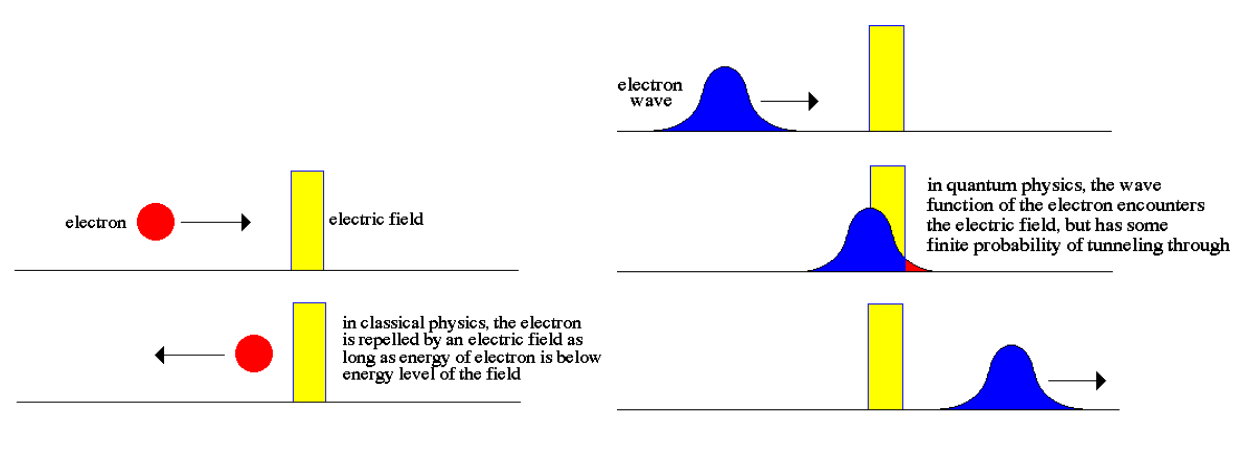
\includegraphics[width=0.5\textwidth]{TunnelingAll.png}
  \end{figure}

% Voor literatuurverwijzingen zijn er twee belangrijke commando's:
% \autocite{KEY} => (Auteur, jaartal) Gebruik dit als de naam van de auteur
%   geen onderdeel is van de zin.
% \textcite{KEY} => Auteur (jaartal)  Gebruik dit als de auteursnaam wel een
%   functie heeft in de zin (bv. ``Uit onderzoek door Doll & Hill (1954) bleek
%   ...'')

%---------- Methodologie ------------------------------------------------------
\section{Methodologie}
\label{sec:methodologie}

Om dit onderzoek te voltooien wordt er een algoritme gezocht die uitvoerbaar is op een klassieke computer.
Dit algoritme wordt dan omgezet naar een quantumalgoritme zodat het ook uitvoerbaar is op een quantumcomputer.
Dan worden er van beide de tijds- en ruimtecomplexiteit berekend. Om te bestuderen wat de effecten zijn van een verhoogd
aantal parameters wordt gezocht naar een algoritme die meer parameters kan accepteren. Dit wordt dan ook uitgevoerd op 
een kleine input (bv in een databank zoeken met een paar duizenden entries) en een grote input (enkele miljoenen entries).
Naast de vergelijking van het algoritme, wordt ook onderzocht naar het effect op de industie. Om dit te kunnen doen wordt er een
vragenlijst opgesteld die beantwoord moet worden door CEO's en CIO's van bedrijven. Uit de vragenlijst moet blijken wat
de belangrijkste bedrijfsprocessen zijn die verbeterd kunnen worden. Van deze processen wordt de complexiteit berekend en
worden deze dan vergeleken met het eerste algoritme. Op basis hiervan wordt dan een schatting gedaan wat het effect zal zijn
als dit proces uitgevoerd zou worden op een quantumcomputer. 

Het berekenen van de tijdscomplexiteit houdt niet veel meer in dan het tellen van het aantal elementaire stappen in het algoritme om dit ten einde te kunnen brengen.
Dit wordt beschreven in \textcite{Abhishek2021Tijd}. Er zijn 3 soorten complexiteit: constant, exponentieel (iets doen in 1 dimensie is lineair, in 2 dimensies kwadratisch enzoverder) of logaritmisch (het werk delen leidt tot een logoaritmische complexiteit).
Geheugen kan voor 3 dingen worden gebruikt: variabelen, de instructies en de executie van het algoritme. Zoals te lezen is in \textcite{Abhishek2021Ruimte} hangt de ruimtecomplexiteit voornamelijk af van het gebruikte geheugen in de executie van het algorimte.
Tijdens het uitvoeren wordt het geheugen op 3 verschillende manieren gebruikt: een deel gaat naar de instructies, een deel gaat naar de systeemstack waar alle variabelen van een algoritme op worden opgeslagen en wachten voor verdere uitvoer en als laatste gaat het geheugen ook naar  de data space (dit is het geheugen dat gebruikt wordt voor de variabelen en constanten).
Het meeste geheugen gaat naar de data space en daarom wordt meestal enkel dit gebruikt om de ruimtecomplexiteit te bereken. Ook in dit onderzoek zal dit zo gebeuren.
Om de ruimtecomplexiteit te bereken, moet er naar het datatype van de variabelen gekeken worden. Zo wordt een boolean bijvoorbeeld in 1 byte opgeslagen en een double in 8 bytes. 
Aan de hand van deze informatie kan de complexiteit gemakkelijk berekend worden.

Om het quantumalgoritme te schrijven en uit te voeren wordt er gebruik gemaakt van IBM's quantumcomputer. IBM heeft een online
tool om quantumalgortimes te maken en dan ook uit te voeren op hun computer.\footnote{\url{https://quantum-computing.ibm.com/}}

%---------- Verwachte resultaten ----------------------------------------------
\section{Verwachte resultaten}
\label{sec:verwachte_resultaten}

Voor de tijdscomplexiteit wordt er een verbetering verwacht die van de orde sqr(n) is.
Bij de ruimtecomplexteit wordt er geen verbetering verwacht aangezien er nog steeds evenveel geheugen nodig is om dezelfde processen uit te voeren.

Enkele van de verwachte voordelen zijn:
\begin{itemize} 
  \item Snellere rendering van complexe 3D-structuren zoals chemische componenten van pillen.
  \item Het sneller maken van meer efficiënte planningen die enkele of zelfs alle processen van een bedrijf voor een gegeven moment bepaald.
  \item Het doorzoeken van grote databanken kan sneller verlopen omdat een quantumcomputer dit in een sqr(n)-tijdsspanne kan doen.
  \item Simulaties van quantumfysica kunnen veel naukeuriger uitgevoerd worden.
  \item Machine learning verloopt veel efficiënter en kan dus voor betere AI-structuren zorgen.
  \item Het ontbinden van in priemfactoren van zeer grote getallen (dit kan de RSA-necryptie helemaal teniet doen).
\end{itemize}
%---------- Verwachte conclusies ----------------------------------------------
\section{Verwachte conclusies}
\label{sec:verwachte_conclusies}

Uit het onderzoek moet een vergelijking blijken tussen een klassieke computer en quantumcomputer. Met deze vergelijking moet er dan onderzocht worden of enkele belangrijke bedrijfsprocessen 
verbeterd kunnen worden door ze uit te voeren op een quantumcomputer. Naast de voordelen van dit zo te doen moet ook gebleken zijn wat de nadelen hiervan zijn.
Zo kan men later bij eventuele implemenaties van quantumcomputers al anticipiëren op de opgesomde nadelen en deze proberen te overbruggen.

%------------------------------------------------------------------------------
% Referentielijst
%------------------------------------------------------------------------------
% TODO: de gerefereerde werken moeten in BibTeX-bestand ``voorstel.bib''
% voorkomen. Gebruik JabRef om je bibliografie bij te houden en vergeet niet
% om compatibiliteit met Biber/BibLaTeX aan te zetten (File > Switch to
% BibLaTeX mode)

\phantomsection
\printbibliography[heading=bibintoc]
\end{document}
